\section{Experimental Data Collection \textbf(SARAH)}
 
SARAH -- expand the experimental description, show map...
\\

Each glider was equipped with a Nortek Signature1000 1 MHz ADCP. Figure \ref{fig.SG} shows an ADCP installed, facing upwards, in the tail section of one of the AUGs. The ADCPs are configured by Nortek to use only three beams---in the upward-facing position, those are the two side beams and the aft beam during descent, and the two side beams and the forward beam during ascent. The ADCPs were programmed to collect a profile every 15 seconds. Each profile covers up to 20 m depth, with a new profile starting approximately every 1.5 m (i.e., the vertical distance covered by the AUG in 15 seconds).
 
 
\begin{figure}[!ht]
  \centering
  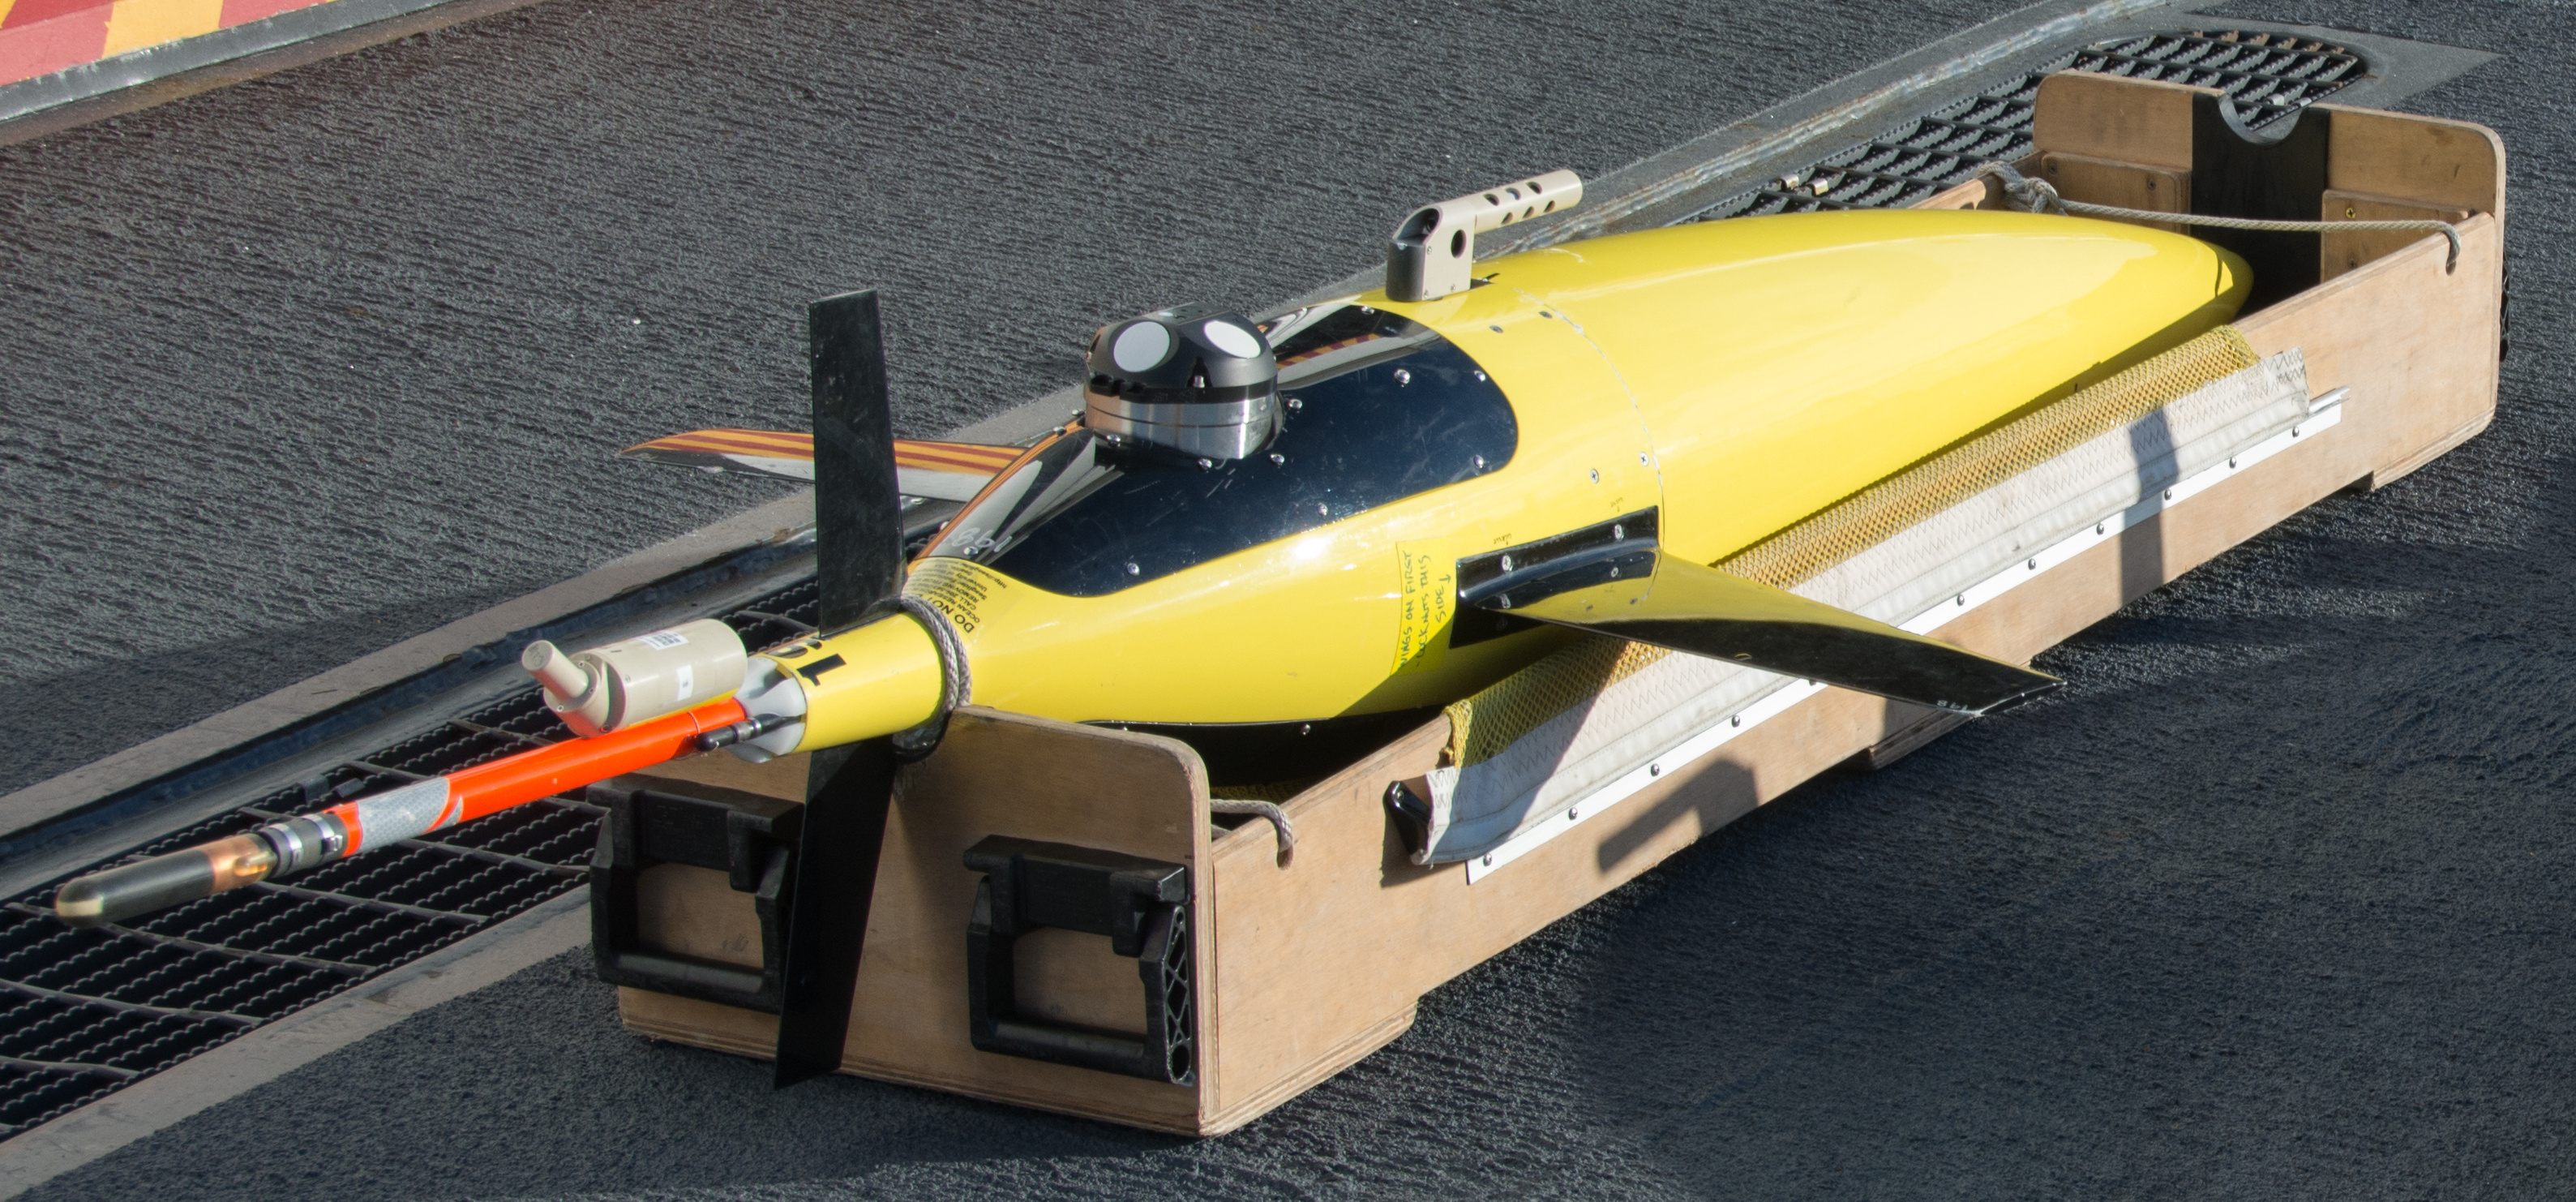
\includegraphics[width=3.0in]{./figs/Gliders_hires-99_crop.jpg}
  %\vspace{-0.1in}
  \caption{Seaglider AUG with an upwards-facing ADCP installed in aft fairing.}
  \label{fig.SG}
%   \vspace{-0.1in}
  %\rule{\textwidth}{0.02in}
  \vspace{-0.2in}
\end{figure}
